%Version 3 December 2023
% See section 11 of the User Manual for version history
%
%%%%%%%%%%%%%%%%%%%%%%%%%%%%%%%%%%%%%%%%%%%%%%%%%%%%%%%%%%%%%%%%%%%%%%
%%                                                                 %%
%% Please do not use \input{...} to include other tex files.       %%
%% Submit your LaTeX manuscript as one .tex document.              %%
%%                                                                 %%
%% All additional figures and files should be attached             %%
%% separately and not embedded in the \TeX\ document itself.       %%
%%                                                                 %%
%%%%%%%%%%%%%%%%%%%%%%%%%%%%%%%%%%%%%%%%%%%%%%%%%%%%%%%%%%%%%%%%%%%%%

%%\documentclass[referee,sn-basic]{sn-jnl}% referee option is meant for double line spacing

%%=======================================================%%
%% to print line numbers in the margin use lineno option %%
%%=======================================================%%

%%\documentclass[lineno,sn-basic]{sn-jnl}% Basic Springer Nature Reference Style/Chemistry Reference Style

%%======================================================%%
%% to compile with pdflatex/xelatex use pdflatex option %%
%%======================================================%%

%%\documentclass[pdflatex,sn-basic]{sn-jnl}% Basic Springer Nature Reference Style/Chemistry Reference Style


%%Note: the following reference styles support Namedate and Numbered referencing. By default the style follows the most common style. To switch between the options you can add or remove “Numbered” in the optional parenthesis. 
%%The option is available for: sn-basic.bst, sn-vancouver.bst, sn-chicago.bst%  
 
%%\documentclass[pdflatex,sn-nature]{sn-jnl}% Style for submissions to Nature Portfolio journals
%%\documentclass[pdflatex,sn-basic]{sn-jnl}% Basic Springer Nature Reference Style/Chemistry Reference Style
\documentclass[pdflatex,sn-mathphys-num]{sn-jnl}% Math and Physical Sciences Numbered Reference Style 
%%\documentclass[pdflatex,sn-mathphys-ay]{sn-jnl}% Math and Physical Sciences Author Year Reference Style
%%\documentclass[pdflatex,sn-aps]{sn-jnl}% American Physical Society (APS) Reference Style
%%\documentclass[pdflatex,sn-vancouver,Numbered]{sn-jnl}% Vancouver Reference Style
%%\documentclass[pdflatex,sn-apa]{sn-jnl}% APA Reference Style 
%%\documentclass[pdflatex,sn-chicago]{sn-jnl}% Chicago-based Humanities Reference Style

%%%% Standard Packages
%%<additional latex packages if required can be included here>

\usepackage{graphicx}%
\usepackage{multirow}%
\usepackage{amsmath,amssymb,amsfonts}%
\usepackage{amsthm}%
\usepackage{mathrsfs}%
\usepackage[title]{appendix}%
\usepackage{xcolor}%
\usepackage{textcomp}%
\usepackage{manyfoot}%
\usepackage{booktabs}%
\usepackage{algorithm}%
\usepackage{algorithmicx}%
\usepackage{algpseudocode}%
\usepackage{listings}%
\usepackage{float}
%%%%

%%%%%=============================================================================%%%%
%%%%  Remarks: This template is provided to aid authors with the preparation
%%%%  of original research articles intended for submission to journals published 
%%%%  by Springer Nature. The guidance has been prepared in partnership with 
%%%%  production teams to conform to Springer Nature technical requirements. 
%%%%  Editorial and presentation requirements differ among journal portfolios and 
%%%%  research disciplines. You may find sections in this template are irrelevant 
%%%%  to your work and are empowered to omit any such section if allowed by the 
%%%%  journal you intend to submit to. The submission guidelines and policies 
%%%%  of the journal take precedence. A detailed User Manual is available in the 
%%%%  template package for technical guidance.
%%%%%=============================================================================%%%%

%% as per the requirement new theorem styles can be included as shown below
\theoremstyle{thmstyleone}%
\newtheorem{theorem}{Theorem}%  meant for continuous numbers
%%\newtheorem{theorem}{Theorem}[section]% meant for sectionwise numbers
%% optional argument [theorem] produces theorem numbering sequence instead of independent numbers for Proposition
\newtheorem{proposition}[theorem]{Proposition}% 
%%\newtheorem{proposition}{Proposition}% to get separate numbers for theorem and proposition etc.

\theoremstyle{thmstyletwo}%
\newtheorem{example}{Example}%
\newtheorem{remark}{Remark}%

\theoremstyle{thmstylethree}%
\newtheorem{definition}{Definition}%

\raggedbottom
%%\unnumbered% uncomment this for unnumbered level heads

\begin{document}

\title[Article Title]{LLMBot: Multi-Agent Robotic Systems for Adaptive Task Execution}

%%=============================================================%%
%% GivenName	-> \fnm{Joergen W.}
%% Particle	-> \spfx{van der} -> surname prefix
%% FamilyName	-> \sur{Ploeg}
%% Suffix	-> \sfx{IV}
%% \author*[1,2]{\fnm{Joergen W.} \spfx{van der} \sur{Ploeg} 
%%  \sfx{IV}}\email{iauthor@gmail.com}
%%=============================================================%%


\author{\fnm{Harith} \sur{Ibrahim}}\email{harithsami01@gmail.com}

\author{\fnm{Harith} \sur{Alsafi}}\email{harith.alsafi@gmail.com}



\affil{\orgdiv{School of Computing}, \orgname{University of Leeds}, \orgaddress{\street{Street}, \city{Leeds}, \postcode{LS2 9JT}, \state{West Yorkshire}, \country{United Kingdom}}}


%%==================================%%
%% Sample for unstructured abstract %%
%%==================================%%

\abstract{This paper presents an innovative approach integrating large language models (LLMs) with robotic systems for natural language interaction and task execution. The proposed system leverages GPT-3.5 Turbo for natural language understanding, reasoning, and high-level task planning, integrated with a simulated 3D environment in Unreal Engine. Behavior trees govern robust low-level execution of robotic actions. The system utilizes prompt engineering, multimodal input, and parameter optimization to enhance the LLM's grounding and performance. Comprehensive evaluation assesses success rates, spatial distributions, and cost-effectiveness across various scenarios. Results demonstrate promising capabilities in executing natural language commands while identifying key limitations. This research advances multi-agent collaboration and human-robot interaction by enabling more intuitive communication between humans and robots. By combining modern language models with classical symbolic AI planners, this project paves the way for more intelligent, adaptive, and cost-effective robotic solutions capable of natural language-based collaboration.}

%%================================%%
%% Sample for structured abstract %%
%%================================%%
 
% \abstract{\textbf{Purpose:} The abstract serves both as a general introduction to the topic and as a brief, non-technical summary of the main results and their implications. The abstract must not include subheadings (unless expressly permitted in the journal's Instructions to Authors), equations or citations. As a guide the abstract should not exceed 200 words. Most journals do not set a hard limit however authors are advised to check the author instructions for the journal they are submitting to.
% 
% \textbf{Methods:} The abstract serves both as a general introduction to the topic and as a brief, non-technical summary of the main results and their implications. The abstract must not include subheadings (unless expressly permitted in the journal's Instructions to Authors), equations or citations. As a guide the abstract should not exceed 200 words. Most journals do not set a hard limit however authors are advised to check the author instructions for the journal they are submitting to.
% 
% \textbf{Results:} The abstract serves both as a general introduction to the topic and as a brief, non-technical summary of the main results and their implications. The abstract must not include subheadings (unless expressly permitted in the journal's Instructions to Authors), equations or citations. As a guide the abstract should not exceed 200 words. Most journals do not set a hard limit however authors are advised to check the author instructions for the journal they are submitting to.
% 
% \textbf{Conclusion:} The abstract serves both as a general introduction to the topic and as a brief, non-technical summary of the main results and their implications. The abstract must not include subheadings (unless expressly permitted in the journal's Instructions to Authors), equations or citations. As a guide the abstract should not exceed 200 words. Most journals do not set a hard limit however authors are advised to check the author instructions for the journal they are submitting to.}

\keywords{Large Language Models, Robotic Systems, Natural Language Interaction, Task Planning, Human-Robot Interaction, Multi-agent Collaboration, Warehouse Automation, Behavior Trees, Simulated Environment, Physical Task Execution, Embodiment}

%%\pacs[JEL Classification]{D8, H51}

%%\pacs[MSC Classification]{35A01, 65L10, 65L12, 65L20, 65L70}
\maketitle


\section{Introduction}\label{sec1}
Intelligent robotic systems have the potential to revolutionize various industries, but developing sophisticated robot planning algorithms has been hindered by high costs and complexity. Recent advancements in natural language processing and large language models (LLMs) present new opportunities for more accessible and cost-effective robot planning.

\begin{figure}[h]
\centering
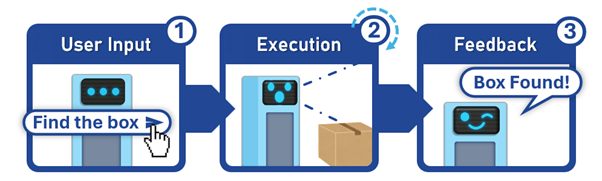
\includegraphics[width=0.6\textwidth]{figures/Picture13.png}
\caption{Diagram Showing Simplified Project Plan}\label{fig1}
\end{figure}
Aim and Objectives
The primary aim of this project is to develop an intelligent virtual robot agent capable of comprehending and executing free-form natural language instructions within a simulated 3D environment. The agent should interpret human commands, reason about the given task, and coherently carry out the necessary actions to accomplish the objective, while exhibiting adaptability to handle novel situations without extensive retraining or reprogramming.

The key objectives include:
\begin{itemize}
    \item Develop an interactive simulation environment for virtual robot agents.
    \item Create virtual agents capable of executing diverse tasks based on natural language input.
    \item Implement an LLM-based robot behavior system for translating natural language instructions into executable behaviors.
    \item Optimize LLM parameters for stable robot embodiment.
    \item Enable robot collaboration and communication within the simulated environment.
    \item Evaluate system performance, running costs, and cost-effectiveness.
\end{itemize}

\section{Background and related work}
\subsection{Large Language Models and Conversational Tuning}
Large Language Models (LLMs) like GPT-3 are neural networks trained on vast amounts of text data, enabling them to generate human-like text outputs. Their training process exposes them to a wide range of knowledge and scenarios, allowing them to exhibit reasoning, common sense, and goal-oriented behaviors. LLMs can be fine-tuned for specific tasks using techniques like prompt engineering and few-shot learning.

\subsection{Embodied Large Language Models}
Recent research has explored techniques to enhance LLMs' capabilities for embodied environments like robotics, including prompt engineering, multimodal prompting, and few-shot learning. These techniques leverage language to define the rules of the world and the robot's abilities, a process called "grounding."

\subsection{Symbolic Planning Methods}
Symbolic planning techniques, such as behavior trees, offer a simple yet powerful way to create adaptable logic and decision-making without the need for complex machine learning models. The proposed approach combines behavior trees with LLMs, leveraging the strengths of both components: LLMs provide rich language understanding capabilities, while symbolic planners offer computational efficiency and the ability to rapidly re-plan lower-level actions based on changes to the symbolic world state.

\begin{figure}[h]
\centering
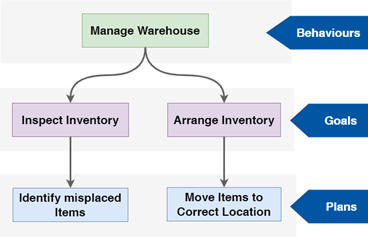
\includegraphics[width=0.6\textwidth]{figures/Picture11.png}
\caption{Example of Behaviour Tree for planning within a warehouse scenario.}\label{fig2}
\end{figure}


\section{Method}
\subsection{Architecture}
The proposed system architecture integrates a Large Language Model (LLM) with robotic agents operating in a virtual Unreal Engine environment. The Python environment handles the LLM's logic, reasoning capabilities, and communication with the simulation via an API. Unreal Engine provides a realistic virtual testbed, leveraging its strengths in intelligent agent creation, behavior simulation, navigation, and perception systems.

\begin{figure}[h]
\centering
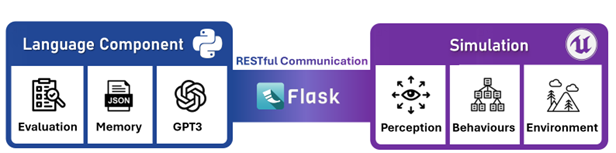
\includegraphics[width=0.7\textwidth]{figures/Picture2.png}
\caption{High level diagram of system architecture.}\label{fig3}
\end{figure}

\textbf{Simulation Environment
}Unreal Engine was chosen as the development platform due to its superior performance, visual quality, and powerful tools for defining and managing intelligent agents' decision-making processes and actions, including its visual scripting system, Blueprints, and its Behavior Tree system.
\begin{figure}[h]
\centering
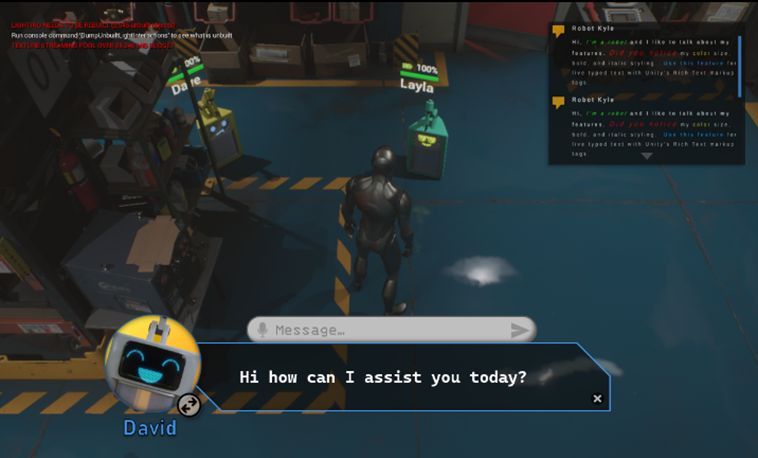
\includegraphics[width=0.6\textwidth]{figures/Picture9.png}
\caption{Screenshot showing Robot Chat User Interface.}\label{fig4}
\end{figure}
\begin{figure}[h]
\centering
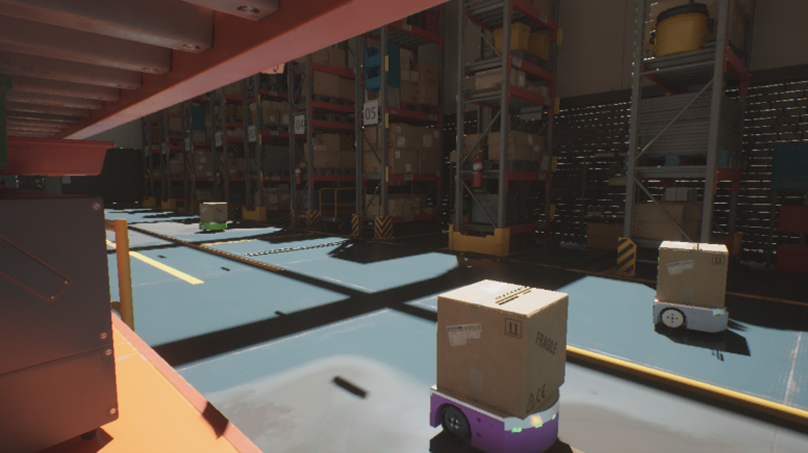
\includegraphics[width=0.6\textwidth]{figures/Picture10.png}
\caption{Screenshot of the simulation. Intelligent robots managing inventory in a Warehouse.}\label{fig5}
\end{figure}
\begin{figure}[H]
\centering
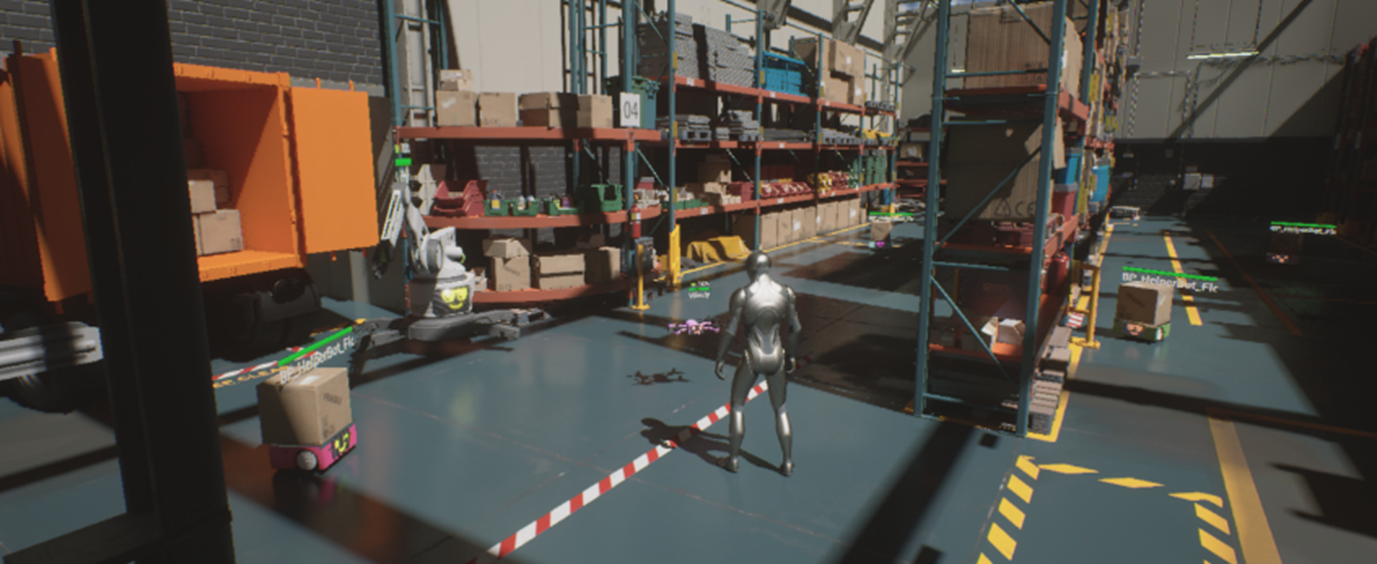
\includegraphics[width=0.6\textwidth]{figures/Picture14.png}
\caption{Warehouse Simulation Environment in Unreal Engine 5.}\label{fig6}
\end{figure}
\begin{algorithm}
\caption{Calculate $y = x^n$}\label{algo1}
\begin{algorithmic}[1]
\Require $n \geq 0 \vee x \neq 0$
\Ensure $y = x^n$ 
\State $y \Leftarrow 1$
\If{$n < 0$}\label{algln2}
        \State $X \Leftarrow 1 / x$
        \State $N \Leftarrow -n$
\Else
        \State $X \Leftarrow x$
        \State $N \Leftarrow n$
\EndIf
\While{$N \neq 0$}
        \If{$N$ is even}
            \State $X \Leftarrow X \times X$
            \State $N \Leftarrow N / 2$
        \Else[$N$ is odd]
            \State $y \Leftarrow y \times X$
            \State $N \Leftarrow N - 1$
        \EndIf
\EndWhile
\end{algorithmic}
\end{algorithm}

\subsection{Language Models and Behaviour Trees}
The system leveraged GPT-3.5 Turbo, a state-of-the-art LLM, for natural language understanding, reasoning, and high-level task planning. Prompting techniques, such as zero and few-shot learning, chain of thought reasoning, and multimodal prompting, were employed to improve the model's performance and grounding in the current environment context.

Behavior trees were used to model and implement decision-making processes in the robotic agents. They offer a hierarchical and modular structure for representing complex behaviors, making them easy to design, debug, and maintain.


\begin{figure}[h]
\centering
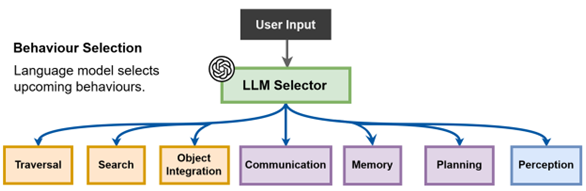
\includegraphics[width=0.6\textwidth]{figures/Picture12.png}
\caption{Proposed approach of utilizing Language Models in Behaviour Trees.}\label{fig7}
\end{figure}

\begin{figure}[h]
\centering
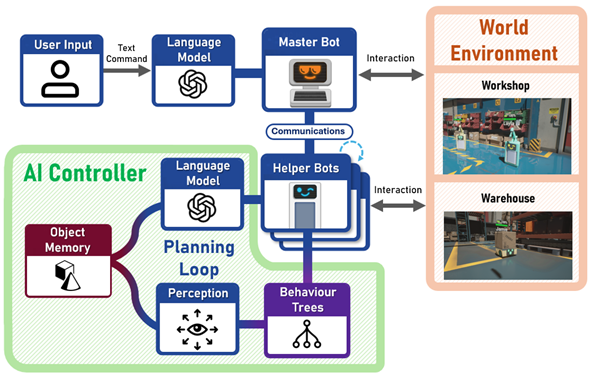
\includegraphics[width=0.9\textwidth]{figures/Picture5.png}
\caption{Proposed Robot Cognitive Architecture.}\label{fig8}
\end{figure}
\subsection{Intelligent System Implementation: Robot Abilities and Communication}

The robotic agents, called HelperBots, could navigate the virtual environment, locate and interact with objects, and perform various tasks based on natural language instructions. They used five high-level behaviors: "Go to" for navigation, "Object interact" for manipulating objects, "Refer to memory" for storing and retrieving environmental information, "Status" for reporting internal status, and "Communicate" for inter-agent communication.


\textbf{Perception and Navigation}
For perception, the system assumed perfect object identification within the robot's line of vision. Regarding navigation, the system utilized Unreal Engine's AI navigation system, employing a technique called Navigation Mesh (NavMesh) for efficient pathfinding in the 3D environment.

\textbf{Robot Memory and Hierarchical Architecture}
The system employed context-aware memory within the language model and object memory on the robot logic side. A "Master Robot" served as a central control unit, with access to the combined memory of all other robots. Several specialized robots, such as DronBot, ArmBot, FloorBot, and ShelfBot, collaborated in a simulated warehouse environment, with the Master Robot coordinating their efforts.
\begin{figure}[h]
\centering
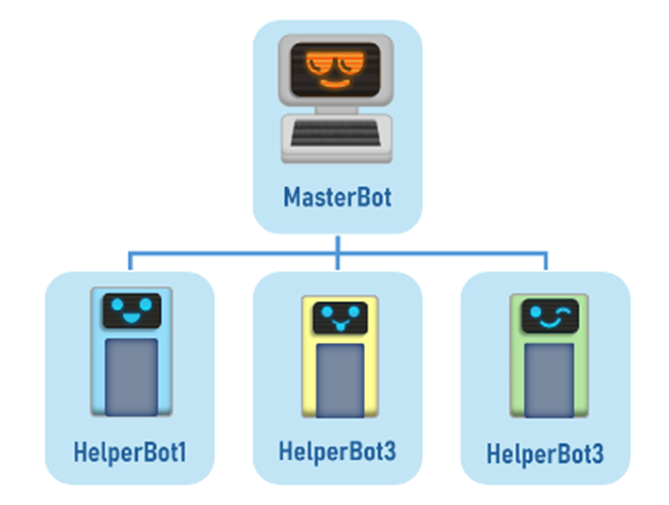
\includegraphics[width=0.5\textwidth]{figures/Picture6.png}
\caption{Diagram of robot command and memory hierarchy.}\label{fig9}
\end{figure}

\textbf{Emotional Intelligence and Real-Life Applications
}The project enhances human-robot interactions by enabling robots to display appropriate emotional expressions based on the chat context. The conversational robot agents have significant potential for real-world applications in various industries, such as collaborative robotics in supermarkets, hospitals, warehouses, factories, office spaces, and care homes.

\textbf{System Modularity}
Modularity and replaceability were emphasized through a JSON file configuration system, decoupling the robot's capabilities from the core system and allowing users to easily swap out or replace individual components without modifying the underlying code.

\section{Experiments}
\subsection{Evaluation Approach}
The evaluation approach aimed to comprehensively assess the system's performance, effectiveness, and the successful blending of classical and modern techniques to enable smooth human-robot collaboration on complex tasks. A general testing environment was developed, simulating a pastry factory operated by a swarm of robots led by a MasterBot. The simulation involved running the environment with multiple robots executing text instructions, using different input parameters for the language model.\cite{benjamin2007cognitive}
\begin{figure}[h]
\centering
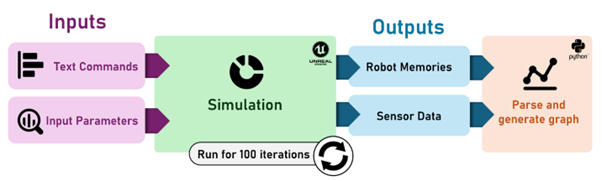
\includegraphics[width=0.8\textwidth]{figures/Picture4.png}
\caption{Simulation Evaluation process diagram.}\label{fig10}
\end{figure}
\subsection{Evaluation Metrics}
The evaluation script analyzed success rates, execution times, individual component performance, battery costs, and the language model running cost. It optimized hyperparameters through over 100 simulation runs and generated a spatial heatmap of robot locations. The analysis provided insights into the system's effectiveness, efficiency, and cost-effectiveness.

\subsection{Results and Discussion}
The robot agents demonstrated an encouraging overall success rate in executing natural language commands, with exceptional performance on conversational tasks. However, room for improvement exists in movement and non-stationary robot tasks. Optimal language model hyperparameters were identified, and spatial analysis revealed even robot distribution without bottlenecks. While longer text inputs slightly decreased success rates, the remarkably low cost for hundreds of API calls highlights the system's economic viability at scale.
\begin{figure}[h]
\centering
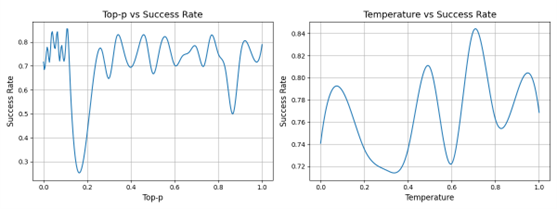
\includegraphics[width=0.9\textwidth]{figures/Picture7.png}
\caption{Success rate plotted against isolated parameters. Top-P (left) and Temperature (right).}\label{fig11}
\end{figure}
\begin{figure}[h]
\centering
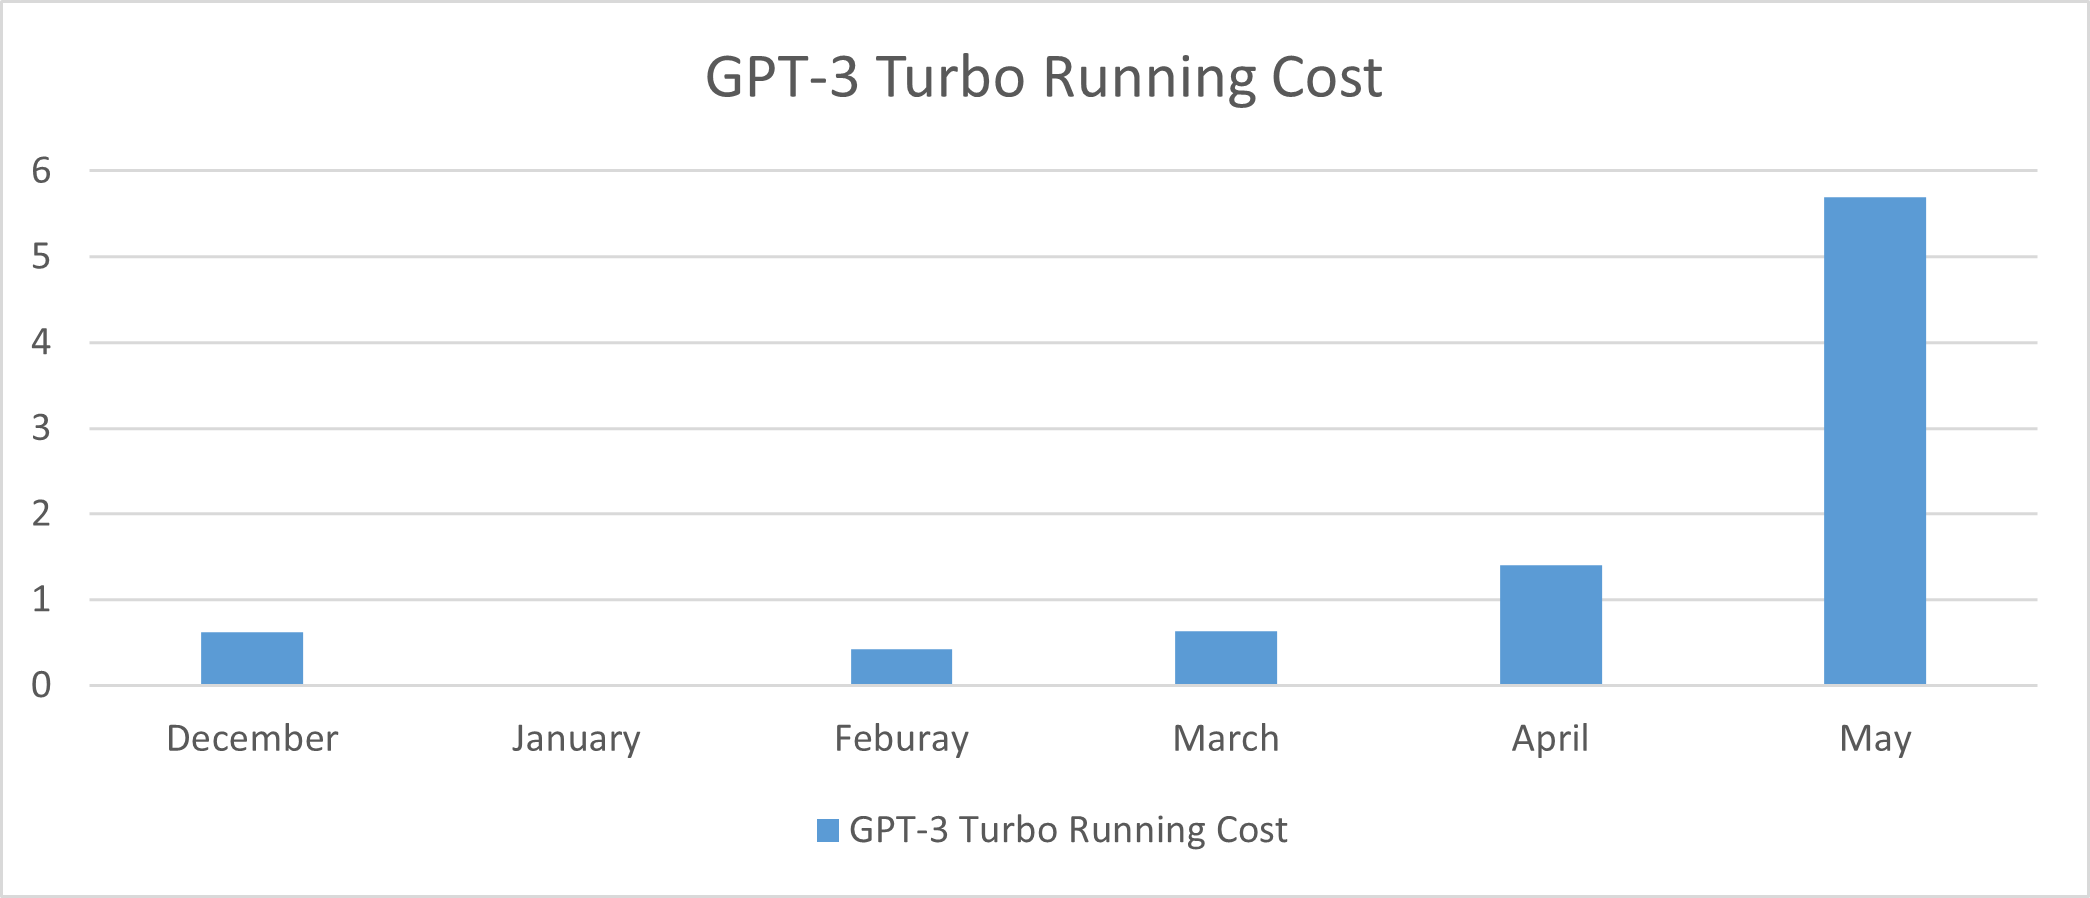
\includegraphics[width=0.9\textwidth]{figures/Picture8.png}
\caption{Language Model API Running Cost.}\label{fig12}
\end{figure}
\begin{figure}[H]
\centering
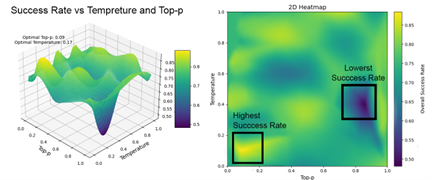
\includegraphics[width=0.9\textwidth]{figures/Picture1.png}
\caption{ Success-Rate plotted against temperature and top-p sampling values.}\label{fig13}
\end{figure} 
\section{Conclusion and Future Work}
% \subsection{Conclusions}
The conversational robot agents project has demonstrated the promising potential of integrating large language models with robotic systems for natural language interaction and task execution. The results highlight the system's viability for real-world applications while identifying areas for improvement. As this technology matures, the integration of natural language processing and cognitive reasoning might revolutionize robot planning and integration across various domains and unlock new frontiers in automation, productivity, and human-robot interaction.

% \subsection{Limitations}
Large language models (LLMs) used in robotics can generate nonsensical or inaccurate outputs, known as hallucinations. These can lead to unintended behaviors, misinterpretations, false assumptions, and confabulation. Providing more context to the model can help mitigate hallucinations, but there is a trade-off between computational cost and the risk of insufficient grounding.

% \subsection{Future Work}
Key future enhancements include transitioning to the Robot Operating System (ROS) framework for real-world robotic hardware testing and deployment, integrating perception and navigation capabilities via real-life sensors, enabling system-generated general subroutines and action loops for task automation in factories and warehouses, and incorporating advanced planning methods like Hierarchical Task Networks (HTN) for efficient execution of complex tasks. Future work should prioritize implementing these advanced planning techniques, ROS integration, and task queuing capabilities.
 
\section*{Acknowledgments}
We would like to acknowledge the support of [funding agency/institution] for providing the resources and funding for this research project. We also express our gratitude to [collaborators/contributors] for their valuable contributions and insights throughout the project's development.


\section*{Declarations}

Some journals require declarations to be submitted in a standardised format. Please check the Instructions for Authors of the journal to which you are submitting to see if you need to complete this section. If yes, your manuscript must contain the following sections under the heading `Declarations':

\begin{itemize}
\item Funding
\item Conflict of interest/Competing interests (check journal-specific guidelines for which heading to use)
\item Ethics approval and consent to participate
\item Consent for publication
\item Data availability 
\item Materials availability
\item Code availability 
\item Author contribution
\end{itemize}

\noindent
If any of the sections are not relevant to your manuscript, please include the heading and write `Not applicable' for that section. 

%%===================================================%%
%% For presentation purpose, we have included        %%
%% \bigskip command. Please ignore this.             %%
%%===================================================%%
\bigskip
\begin{flushleft}%
Editorial Policies for:

\bigskip\noindent
Springer journals and proceedings: \url{https://www.springer.com/gp/editorial-policies}

\bigskip\noindent
Nature Portfolio journals: \url{https://www.nature.com/nature-research/editorial-policies}

\bigskip\noindent
\textit{Scientific Reports}: \url{https://www.nature.com/srep/journal-policies/editorial-policies}

\bigskip\noindent
BMC journals: \url{https://www.biomedcentral.com/getpublished/editorial-policies}
\end{flushleft}

\begin{appendices}

\section{Section title of first appendix}\label{secA1}

An appendix contains supplementary information that is not an essential part of the text itself but which may be helpful in providing a more comprehensive understanding of the research problem or it is information that is too cumbersome to be included in the body of the paper.

%%=============================================%%
%% For submissions to Nature Portfolio Journals %%
%% please use the heading ``Extended Data''.   %%
%%=============================================%%

%%=============================================================%%
%% Sample for another appendix section			       %%
%%=============================================================%%

%% \section{Example of another appendix section}\label{secA2}%
%% Appendices may be used for helpful, supporting or essential material that would otherwise 
%% clutter, break up or be distracting to the text. Appendices can consist of sections, figures, 
%% tables and equations etc.

\end{appendices}

%%===========================================================================================%%
%% If you are submitting to one of the Nature Portfolio journals, using the eJP submission   %%
%% system, please include the references within the manuscript file itself. You may do this  %%
%% by copying the reference list from your .bbl file, paste it into the main manuscript .tex %%
%% file, and delete the associated \verb+\bibliography+ commands.                            %%
%%===========================================================================================%%

\bibliography{sn-bibliography}% common bib file
%% if required, the content of .bbl file can be included here once bbl is generated
%%\input sn-article.bbl

\end{document}